\chapter{Ejemplo de utilización de la aplicación}

Para mostrar el funcionamiento de este trabajo fin de grado gráficamente, a continuación se explica el ejemplo de un caso práctico con todos los pasos seguidos y los resultados obtenidos. 

\section{Caso práctico}

Se supone un usuario que va a solicitar un estudio sobre cuatro páginas de Facebook relacionadas con compañías telefónicas.

\begin{itemize}
\item \textbf{PASO 1: Registro en la aplicación}\\
Se registra en la aplicación como un nuevo usuario. Se llama usuarioPrueba. En la siguiente figura se muestra este paso una vez completado y creado satisfactoriamente.
\begin{figure}[H]
\centering
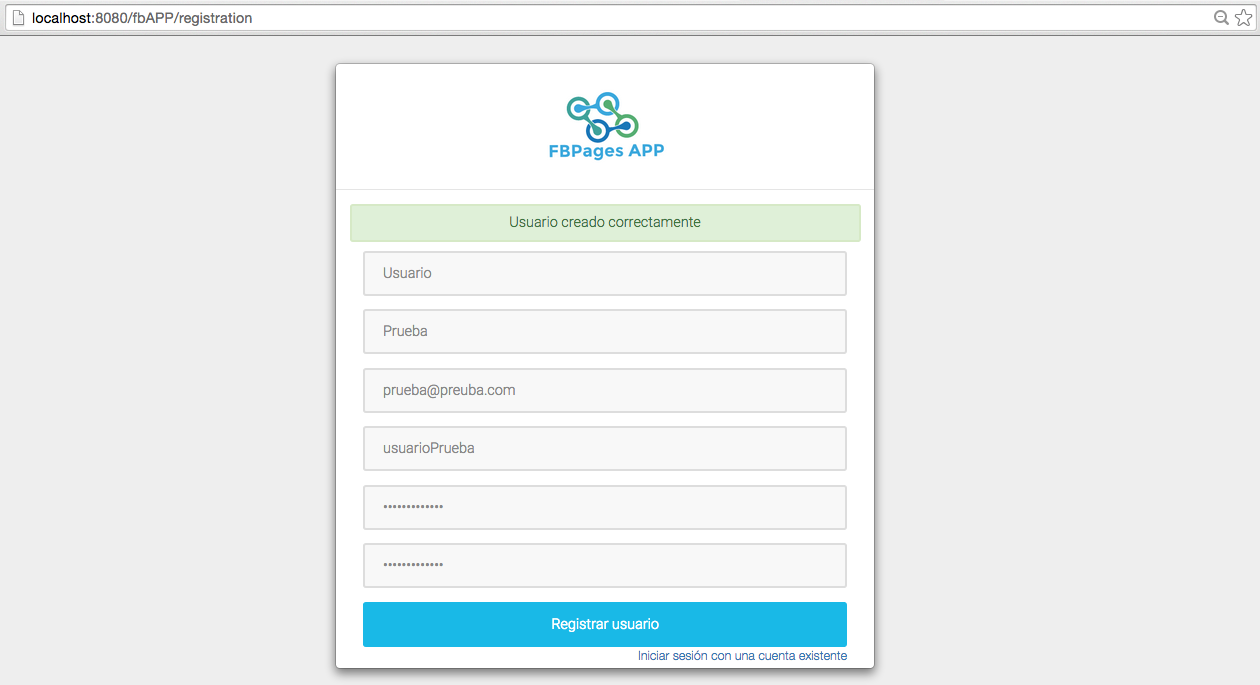
\includegraphics[width=5.5in]{figuras/ejemploRegistro.png}
\caption{Captura de pantalla ejemplo Registro de usuario} \label{fig:exregistro}
\end{figure}
\item \textbf{PASO 2: Inicio de sesión}\\
Una vez creado el usuario, ya puede acceder a la aplicación con el nombre de usuario y contraseña establecidos. A continuación se presenta un ejemplo de este paso gráficamente. 
\begin{figure}[H]
\centering
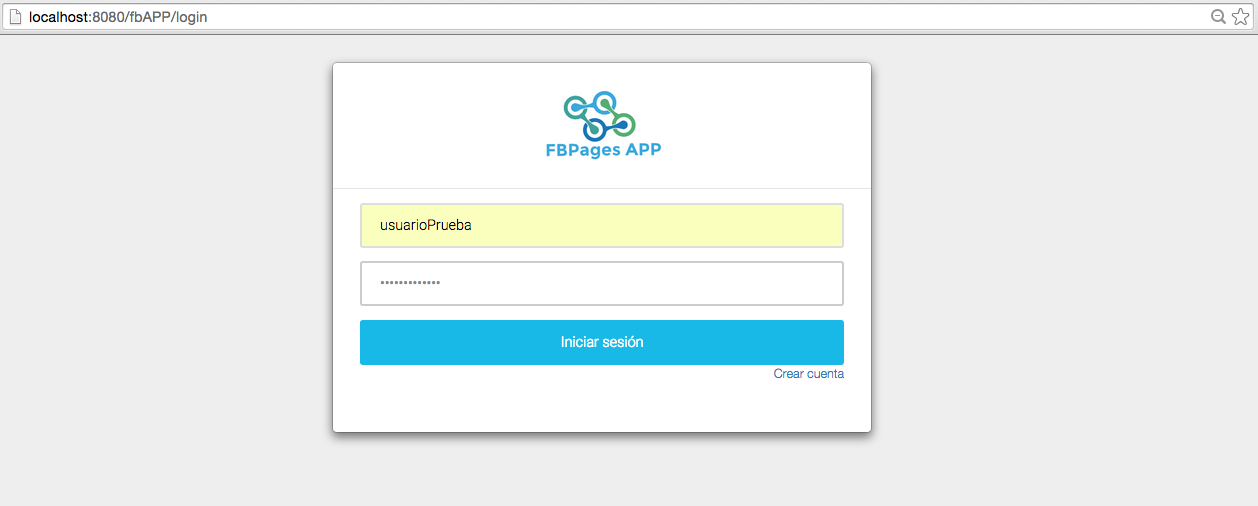
\includegraphics[width=5in]{figuras/ejemploLogin.png}
\caption{Captura de pantalla ejemplo Inicio de sesión} \label{fig:exlogin}
\end{figure}
\item \textbf{PASO 3: Solicitud del análisis a realizar}
El siguiente paso se divide en cuatro. Consiste en definir las características del análisis de que va a realizar.
\begin{enumerate}
\item En el primer formulario hay que indicar el nombre que va a englobar el estudio. En este caso, Compañías telefónicas. 
\begin{figure}[H]
\centering
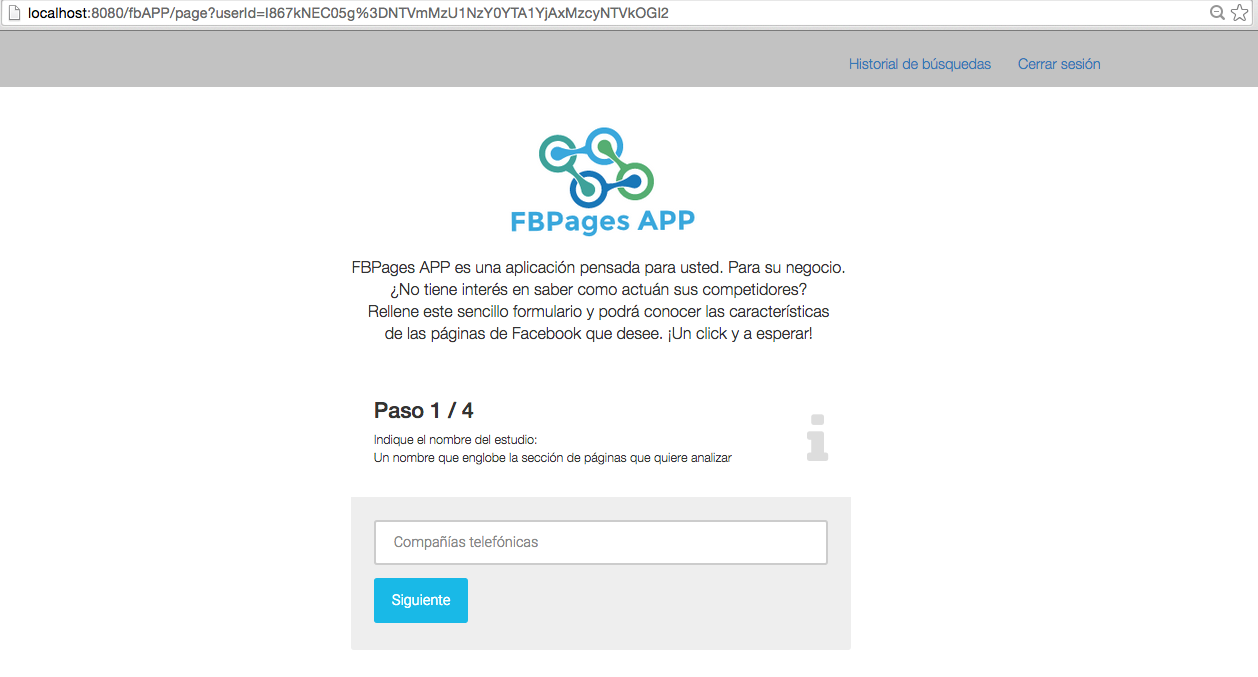
\includegraphics[width=5in]{figuras/ejemploPaso1.png}
\caption{Captura de pantalla ejemplo solicitud de análisis. Paso 1} \label{fig:exPaso1}
\end{figure}
\item En el segundo hay que indicar el nombre de las páginas de Facebook que se van a analizar. En este caso práctico, se quien analizar las páginas de las compañías telefónicas Movistar, Orange, Vodafone y Jazztel. 

No es suficiente con poner el nombre de la compañía, hay que introducir el nombre que Facebook indica en la dirección URL. Para ello, se ha buscado la página de Movistar, a modo de ejemplo. Como es una compañía internacional, hay varias páginas posibles para esta búsqueda, en este caso, se va a elegir Movistar España.  En la siguiente figura se muestra la búsqueda en Facebook para entenderlo mejor.
\begin{figure}[H]
\centering
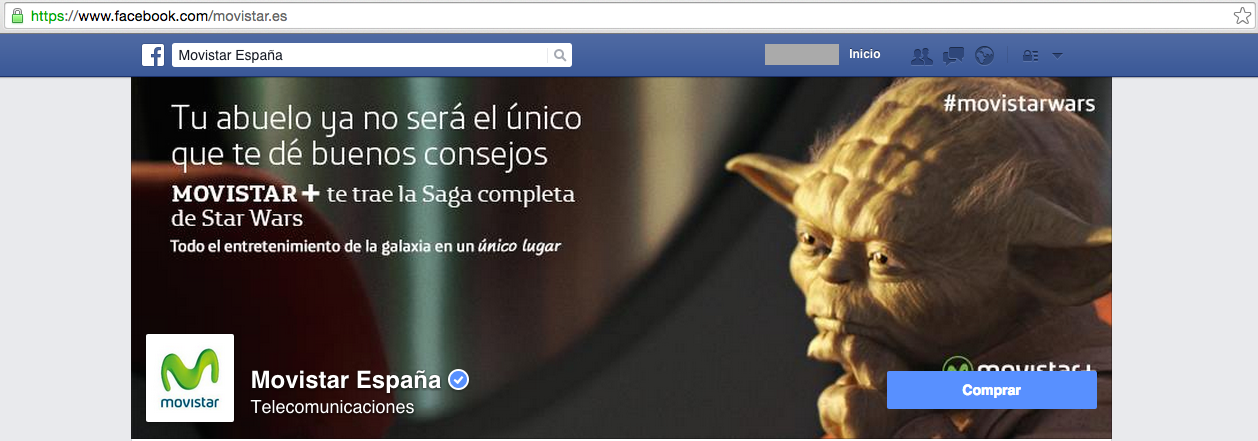
\includegraphics[width=5in]{figuras/ejemploFacebook.png}
\caption{Captura de pantalla ejemplo búsqueda en Facebook} \label{fig:exFacebook}
\end{figure}
Además de elegir la página adecuada para los requisitos esperados del estudio, es conveniente comprobar que existe la sección \textit{Post to Page} de la página seleccionada. Este paso se realiza añadiendo al final de la URL el texto "/posts\_to\_page", y si se carga una pantalla mostrando las publicaciones de los usuarios, significa que existe. A continuación se muestra gráficamente.
\begin{figure}[H]
\centering
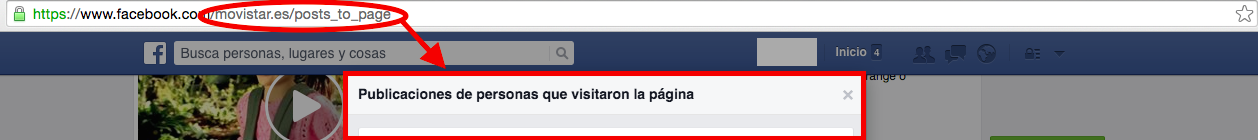
\includegraphics[width=5in]{figuras/ejemploPostToPage.png}
\caption{Captura de pantalla ejemplo comprobación sección \textit{Post to Page}} \label{fig:exPostToPage}
\end{figure}
Una vez realizadas las comprobaciones necesarias para las cuatro compañías telefónicas se introducen con el nombre adecuado en el formulario, tal y como se muestra en la siguiente figura.
\begin{figure}[H]
\centering
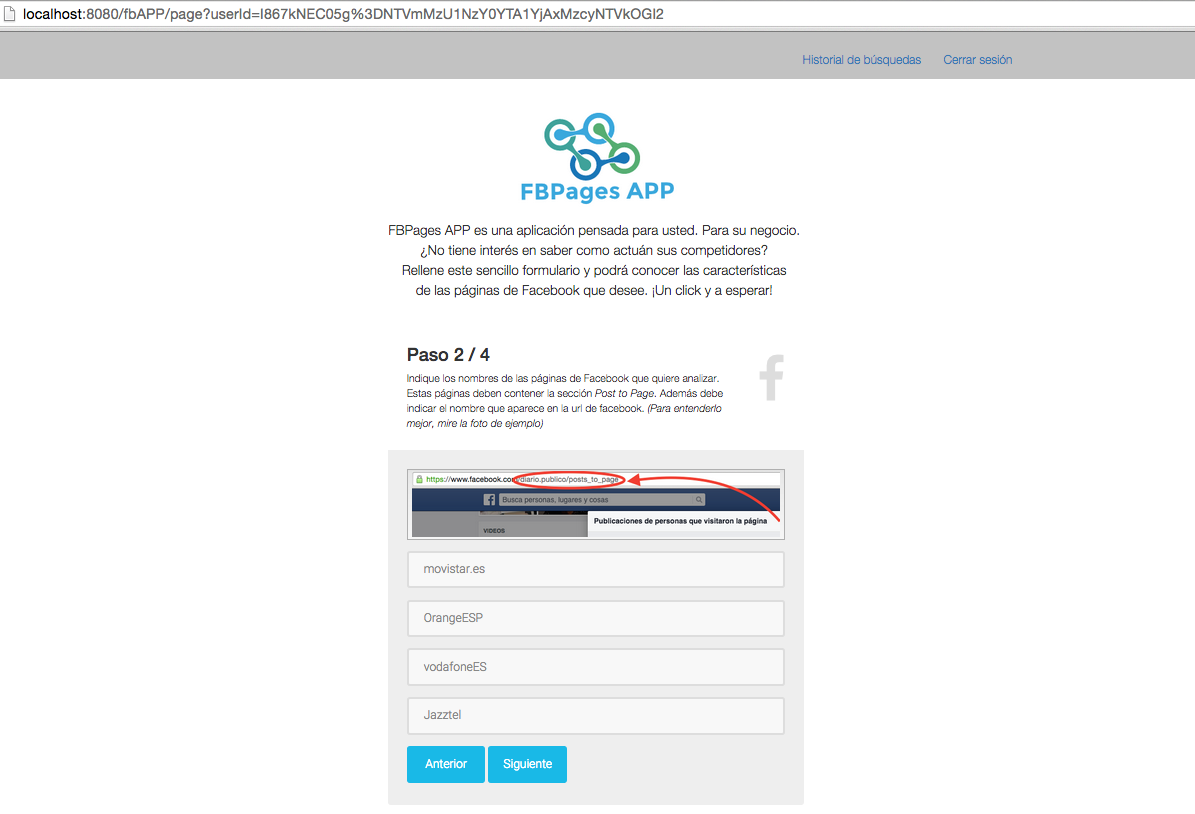
\includegraphics[width=5in]{figuras/ejemploPaso2.png}
\caption{Captura de pantalla ejemplo solicitud de análisis. Paso 2} \label{fig:exPaso2}
\end{figure}
\item En el tercer paso, hay que indicar el periodo temporal del estudio a realizar. En concreto se quiere realizar del último año, por lo que se introducirá la fecha de inicio el uno de septiembre de 2014, en el formato indicado por la aplicación.
\begin{figure}[H]
\centering
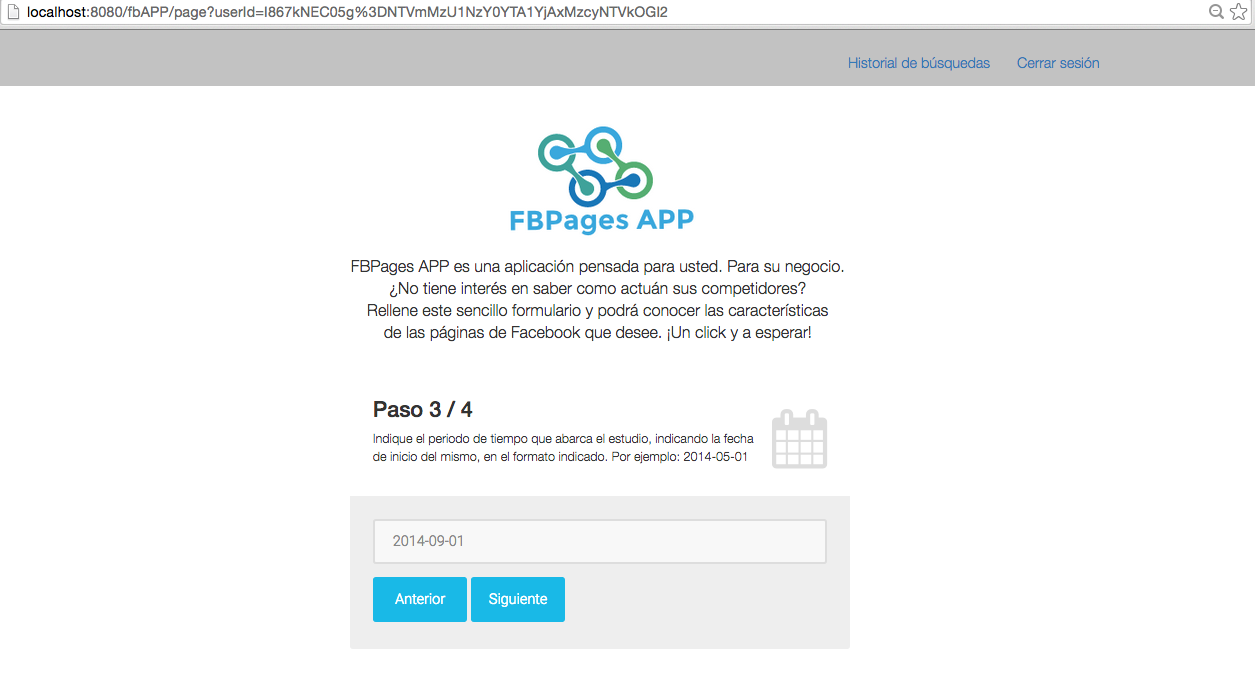
\includegraphics[width=5in]{figuras/ejemploPaso3.png}
\caption{Captura de pantalla ejemplo solicitud de análisis. Paso 3} \label{fig:exPaso3}
\end{figure}
\item Por último, se debe indicar una dirección de correo electrónico a la que se avisará una vez finalizado el estudio de Facebook, además de seleccionar las características del análisis. En este caso se van a seleccionar ambas, "Informe de las páginas" e "Informe de los usuarios de las páginas". 
\begin{figure}[H]
\centering
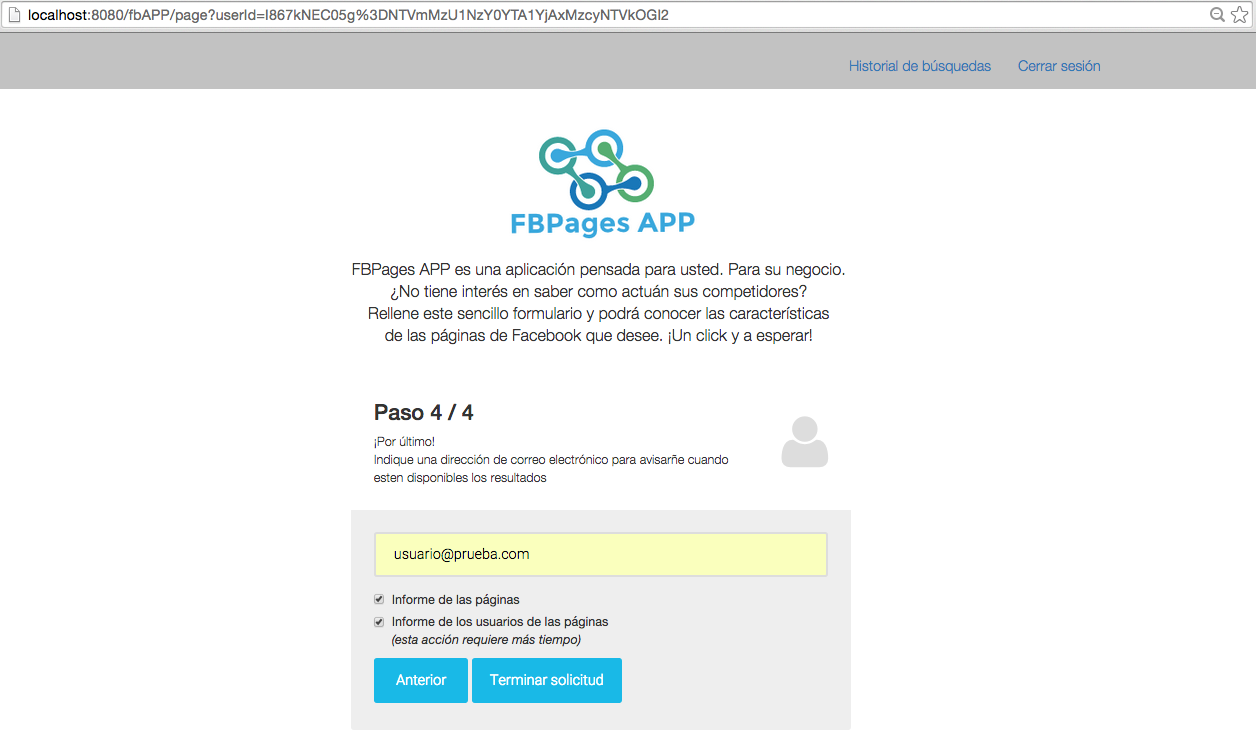
\includegraphics[width=5in]{figuras/ejemploPaso4.png}
\caption{Captura de pantalla ejemplo solicitud de análisis. Paso 4} \label{fig:exPaso4}
\end{figure}
Una vez completados todos los formularios necesarios para realizar una solicitud de un análisis, se pulsa en el botón "Terminar solicitud".
\end{enumerate}
\item \textbf{PASO 4: Tiempo de espera hasta que llegue la notificación por correo}\\
Después de pulse el botón "Terminar solicitud", se visualiza la pantalla que se muestra a continuación. En la que se indica al usuario que debe esperar a que se haya realizado el análisis de las páginas de Facebook.
\begin{figure}[H]
\centering
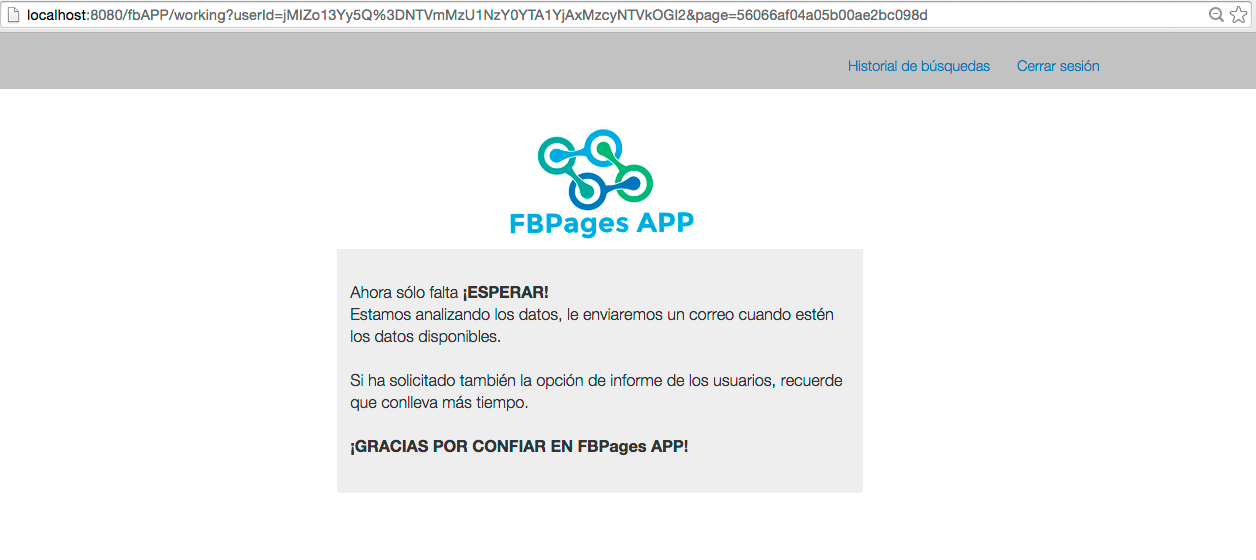
\includegraphics[width=5in]{figuras/ejemploWorking.png}
\caption{Captura de pantalla ejemplo pantalla de espera} \label{fig:exWorking}
\end{figure}

Pasado el tiempo necesario para obtener los datos del análisis, el usuario recibe un correo donde se le avisa de que ya puede ver los resultados del estudio. En la siguiente imagen, se muestra un ejemplo del correo recibido.

\begin{figure}[H]
\centering
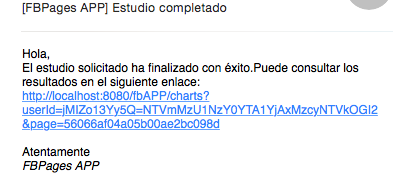
\includegraphics[width=5in]{figuras/ejemploCorreo.png}
\caption{Captura de pantalla ejemplo correo recibido} \label{fig:exCorreo}
\end{figure}

\item \textbf{PASO 5: Visualización de los resultados}
Pinchando en el enlace indicado en el correo recibido (Figura \ref{fig:exCorreo}) se pueden ver los resultados. Otra opción es acceder de nuevo a la aplicación y pulsar sobre la opción "Historial de búsquedas", donde aparece una tabla que recoge todos los análisis solicitados y se selecciona la opción "Ver análisis". En la siguiente figura se muestra el Historial de Búsquedas del usuarioPrueba. 
\begin{figure}[H]
\centering
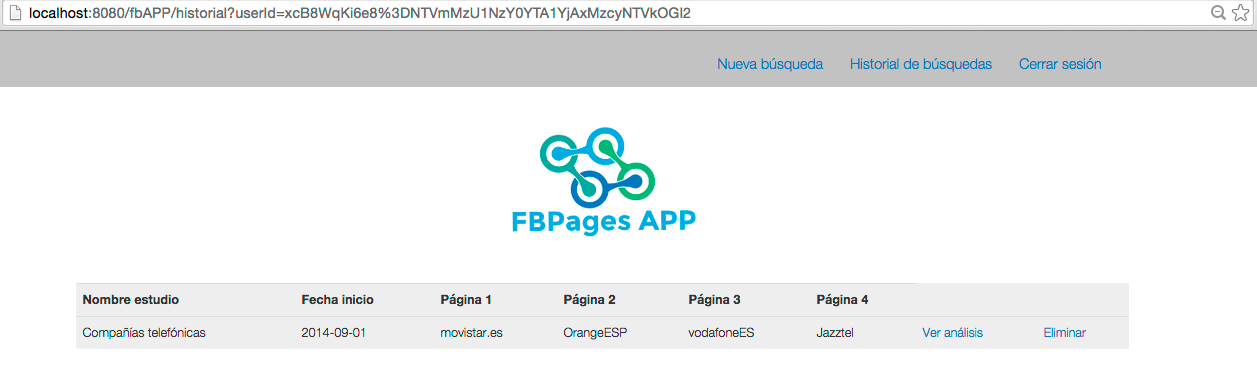
\includegraphics[width=5in]{figuras/ejemploHistorialUser.png}
\caption{Captura de pantalla ejemplo historial de búsquedas del usuario} \label{fig:exHistorial}
\end{figure}

Por último, para finalizar la explicación de este caso práctico, se presentan los resultados que ha obtenido el usuario después de todo el proceso.

Dado que el análisis de los usuarios requiere más tiempo, si el usuario accede automáticamente después de recibir el correo, sólo ve el análisis de las páginas de Facebook, y el análisis de los usuarios en espera. Tal y como se muestra en la siguiente figura. 
\begin{figure}[H]
\centering
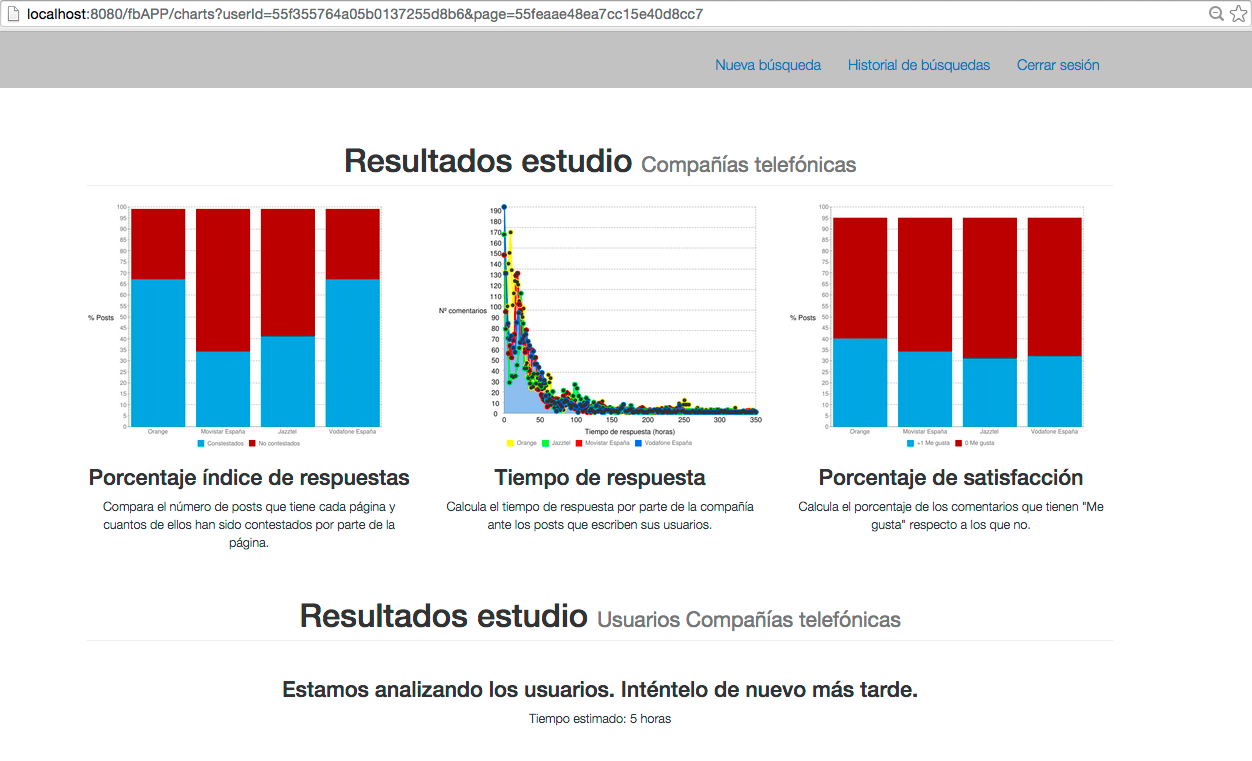
\includegraphics[width=5in]{figuras/ejemploAnalisisFB.png}
\caption{Captura de pantalla ejemplo análisis obtenido. Sólo las páginas} \label{fig:exAnalisisFB}
\end{figure}
Si transcurrido un tiempo vuelve a acceder a la aplicación, ya estarán disponibles los resultados de los usuarios, visualizando el análisis completo.
\begin{figure}[H]
\centering
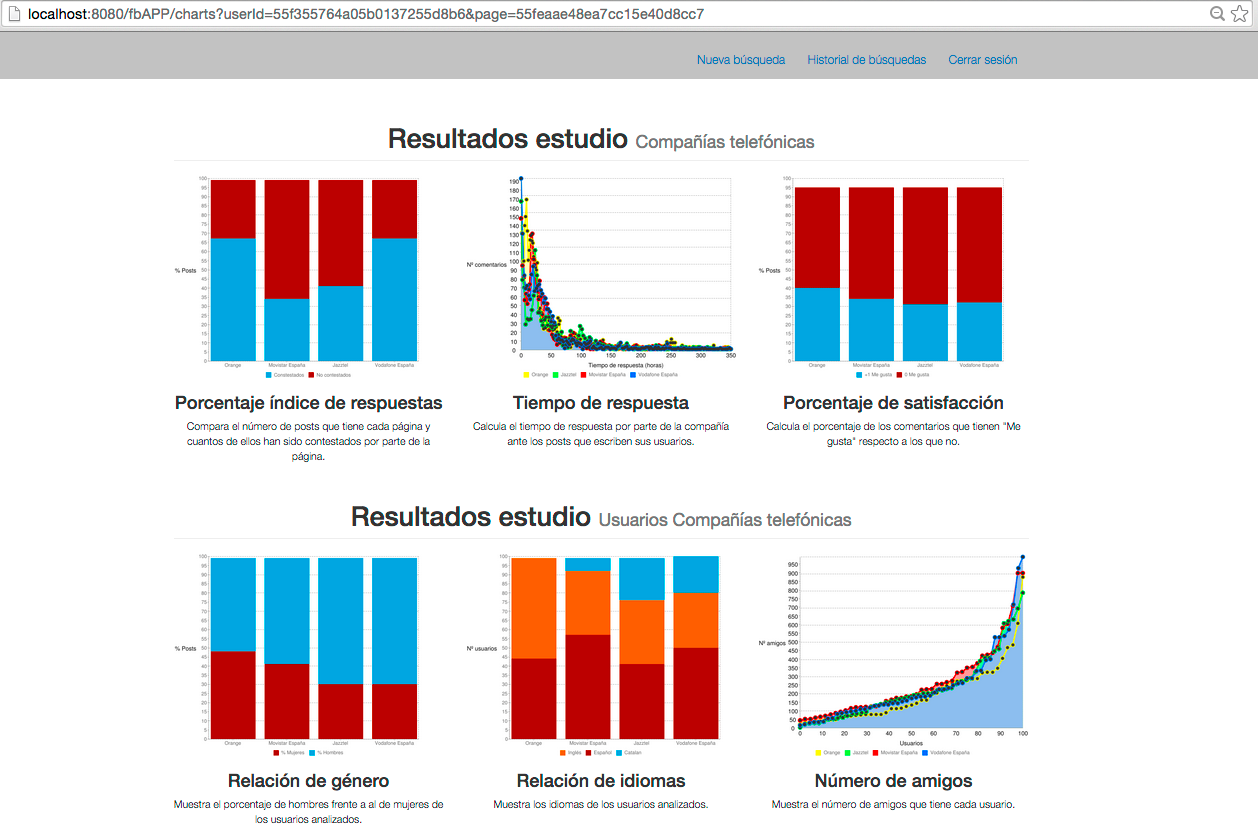
\includegraphics[width=5in]{figuras/ejemploAnalisis.png}
\caption{Captura de pantalla ejemplo análisis obtenido. Completo} \label{fig:exAnalisis}
\end{figure}
\end{itemize}